\graphicspath{ {project_images/} }

\section{Evaluation}
Evaluation of our models involved analyzing the following metrics:

\begin{itemize}
	\item Test accuracy
	\begin{itemize}
		\item Measures how well the model makes correct predictions on data it has not seen before in training.
	\end{itemize}
	\item Precision score
	\begin{itemize}
		\item Measures how many positive predictions are true positives.
	\end{itemize}
	\item Recall score
	\begin{itemize}
		\item Measures how well the model predicts all positive instances.
	\end{itemize}
	\item F1 score
	\begin{itemize}
		\item Measure the mean between precision and recall.
		\item This is especially useful since our dataset has a different amount of instances of each class. 
	\end{itemize}
\end{itemize}

We also referred to a confusion matrix for each model that summarized how well classification was executed. Figure \ref{fig:figure3} below demonstrates the value of the elements of a multi-class confusion matrix from the perspective of the first class.

\begin{figure}[h]
	\centering
	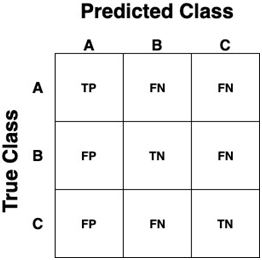
\includegraphics[scale=0.4]{multiclass_cfm}
	\caption{Multi-Class Confusion Matrix}
	\label{fig:figure3}
\end{figure}

When analyzing the first class, TP represent true positive instances, TN true negative instances, FP false positive instances, and FN false negative instances.

\subsection{SVM}

SVM took a long time to run when looking at all the data, resulting in several days to compute a single model.
By using Grid Search to find the best hyperparameter values, we were able to compute the following Confusion Matrix.
However, this model was severely overfitting as seen in \ref{fig:figure19}.
It was decided that instead of trying to work with SVM which would take a long time to compute the model, we would focus more so on the various CNN algorithms.
The best hyperparameters found to compute the following results were $C = 10$ and $\gamma = \frac{1}{250,001}$.

\begin{figure}[h]
    \begin{subfigure}{0.4\textwidth}
        \centering
        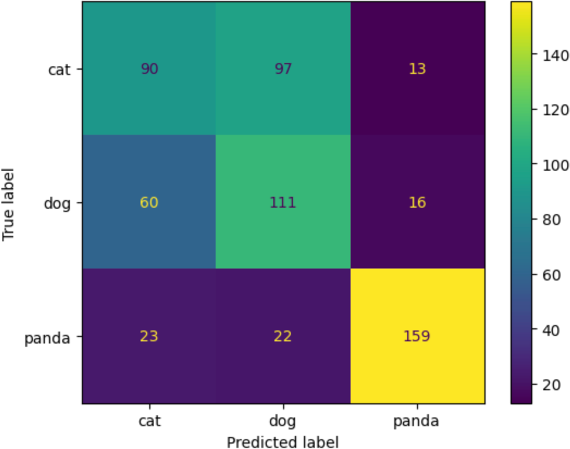
\includegraphics[scale=0.5]{csvm_cfm}
        \caption{Confusion Matrix of SVM}
        \label{fig:figure3}
    \end{subfigure}
    \hspace{0.2\textwidth}
	\begin{subfigure}{0.4\textwidth}
        \centering
        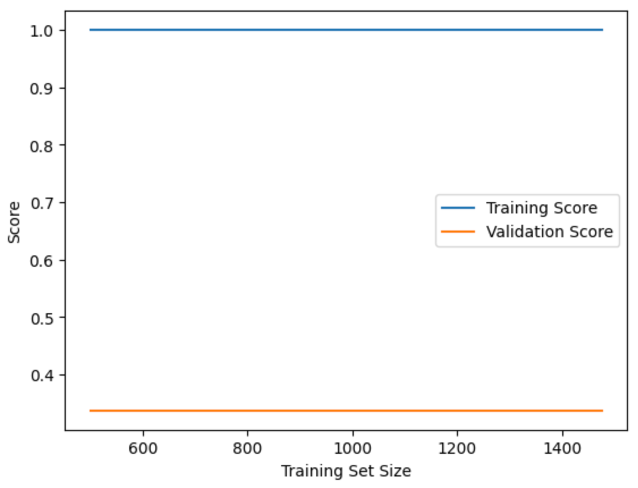
\includegraphics[scale=0.5]{svm_overfit}
        \caption{Confusion Matrix of SVM}
        \label{fig:figure19}
    \end{subfigure}
\end{figure}

\subsection{CNN}
The first few training runs were done on a simpler CNN model with less convoluted and max-pooling layers. While run time was fairly quick, performance was low as the model was too simple. We experimented with adding more convoluted and max-pooling layers and found that adding too many made training time too long considering that performance did not improve much. The final structure is what we found to be the most efficient training-time wise for our project while also considering performance. Most runs averaged between 50-60\% accuracy before applying data augmentation and improved to 60-70\% after applying data augmentation. Our final run reached about 76\% test accuracy with a 76\% precision score, 76\% recall score, and a 75\% f1 score. The confusion matrix for our final CNN run is shown in Figure \ref{fig:figure4} below.

\begin{figure}[h]
	\centering
	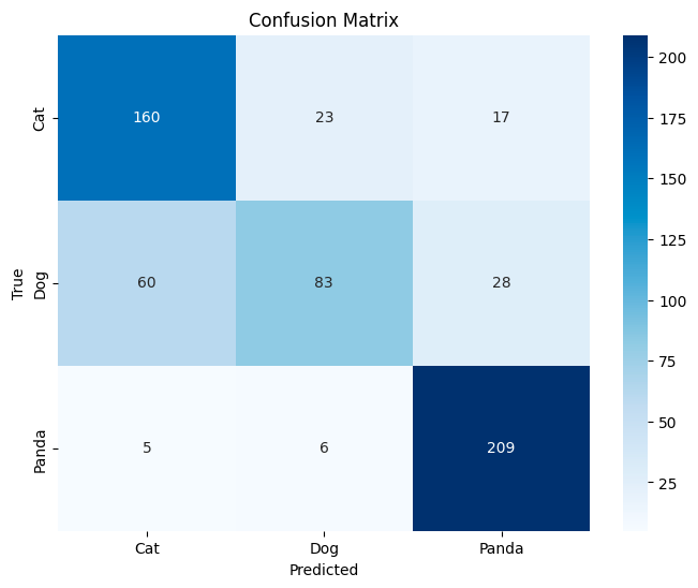
\includegraphics[scale=0.5]{CNN_cfm}
	\caption{Confusion matrix for final CNN run. The model consistently had the most difficulty classifying dogs and the most success classifying pandas.}
	\label{fig:figure4}
\end{figure}

\subsection{ResNet50}

There were several models that were made in order to get better results.
The models used differing amounts of hidden layers, dropout, Conv2D, and MaxPooling2D layers.
We found that the best perfoming model was a simple structure with a single hidden layer with a dropout of 20\%.
This model yielded an accuracy of 61\%.

\begin{figure}[h]
    \begin{subfigure}{0.4\textwidth}
        \centering
        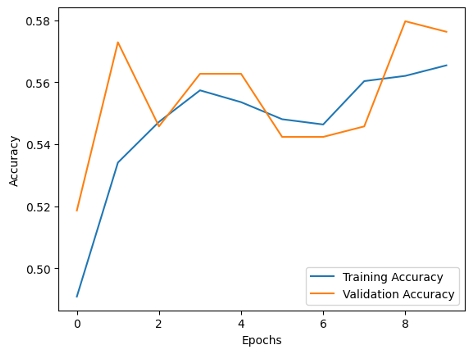
\includegraphics[scale=0.5]{resnet50_acc}
        \caption{Res Net 50: Accuracy vs Epochs}
        \label{fig:figure3}
    \end{subfigure}
    \hspace{0.2\textwidth}
    \begin{subfigure}{0.4\textwidth}
        \centering
        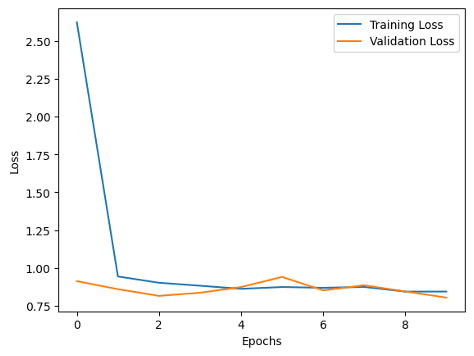
\includegraphics[scale=0.5]{resnet50loss}
        \caption{Res Net 50: Loss vs Epochs}
        \label{fig:figure3}
    \end{subfigure}
\end{figure}

\subsection{VGG16}
The first training run was done with 3 dense layers manually added on top of the pre-trained VGG16 model and took approximately 14 hours to run through 15 epochs (there were 25 total epochs but the EarlyStopping callback was implemented which stopped training after 15 epochs). This first run yielded about 50\% accuracy and after experimenting with different hyperparameter values, it was apparent that the long run time could be shortened by removing a dense layer to decrease the complexity of the model without sacrificing performance too much. This is most likely because our dataset is small compared to what the VGG16 model was pre-trained on, and so an increase in complexity did not increase performance as the model struggled learn stably. Reducing the number of dense layers to 2 decreased training time to approximately 18 minutes per epoch (as opposed to 1 hour and 20 minutes per epoch before removing the third dense layer). Most runs stayed between 50-60\% with and without data augmentation. Our final run scored about 55\% on test accuracy, 58\% on precision, 55\% on recall, and 49\% on f1. The confusion matrix for our final VGG16 run is shown in Figure\ref{fig:figure5} below, where a significant number of false predictions can be observed. 

\begin{figure}[h]
	\centering
	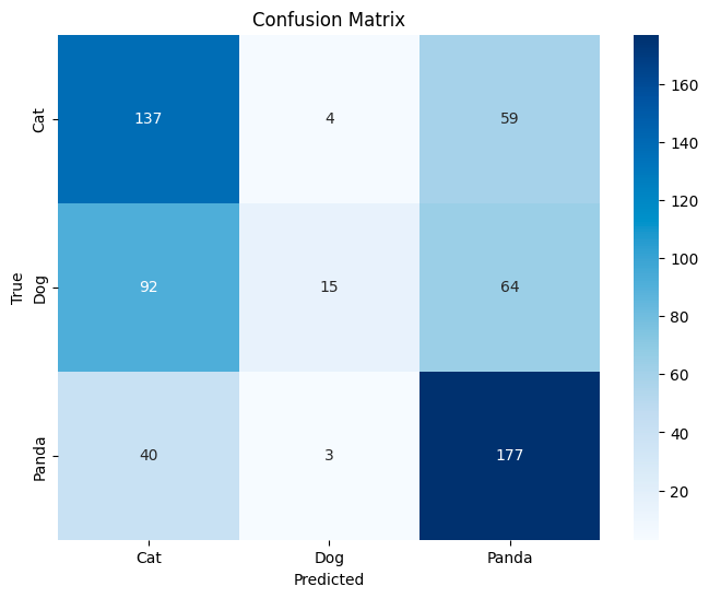
\includegraphics[scale=0.5]{VGG16_cfm}
	\caption{Confusion matrix for final VGG16 run.}
	\label{fig:figure5}
\end{figure}